% ****** Start of file apssamp.tex ******
%
%   This file is part of the APS files in the REVTeX 4.1 distribution.
%   Version 4.1r of REVTeX, August 2010
%
%   Copyright (c) 2009, 2010 The American Physical Society.
%%%%%%%%%%%%%%%%%%%%%%%%%%%%%%%%%%%%%%%%%%%%%%%%%%%%%%%%%%%%%%%%%%%%%%%%%%%%%%%%
%   Modified for use as qtdsp.tex
%
%   See the REVTeX 4 README file for restrictions and more information.
%
% TeX'ing this file requires that you have AMS-LaTeX 2.0 installed
% as well as the rest of the prerequisites for REVTeX 4.1
%
% See the REVTeX 4 README file
% It also requires running BibTeX. The commands are as follows:
%
%  1)  latex apssamp.tex
%  2)  bibtex apssamp
%  3)  latex apssamp.tex
%  4)  latex apssamp.tex
%
\documentclass[%
 reprint,
%superscriptaddress,
%groupedaddress,
%unsortedaddress,
%runinaddress,
%frontmatterverbose,
%preprint,
%showpacs,preprintnumbers,
%nofootinbib,
%nobibnotes,
%bibnotes,
 amsmath,amssymb,
 aps,
 pra,
%prb,
%rmp,
%prstab,
%prstper,
%floatfix,
 longbibliography
]{revtex4-1}

\usepackage{graphicx}% Include figure files
%\usepackage{bm}% bold math
\usepackage{gensymb}
%\usepackage{hyperref}% add hypertext capabilities
%\usepackage[mathlines]{lineno}% Enable numbering of text and display math
%\linenumbers\relax % Commence numbering lines

%\usepackage[showframe,%Uncomment any one of the following lines to test
%%scale=0.7, marginratio={1:1, 2:3}, ignoreall,% default settings
%%text={7in,10in},centering,
%%margin=1.5in,
%%total={6.5in,8.75in}, top=1.2in, left=0.9in, includefoot,
%%height=10in,a5paper,hmargin={3cm,0.8in},
%]{geometry}

%%%%%%%%%%%%%%%%%%%%%%%%%%%%%%%%%%%%%%%%%%%%%%%%%%%%%%%%%%%%%%%%%%%%%%%%%%%%%%%%
%%%%  Body of document follows...
%%%%%%%%%%%%%%%%%%%%%%%%%%%%%%%%%%%%%%%%%%%%%%%%%%%%%%%%%%%%%%%%%%%%%%%%%%%%%%%%
\begin{document}

\preprint{APS/123-QED}

\input{../source/qtdsp_title}
\begin{abstract}
Consciousness can be considered a physical process occurring inside and outside of time simultaneously,
per spiritual traditions and modern QM theory, using two-dimensional time.
In this model, quantum time emerges from non-local consciousness as it interacts with both worlds.
The relationship between the time dimensions provides a mechanism for apparent
noise arising from both our biological signaling and connection to a timeless divinity.
We present an algorithm for the demodulation of ubiquitous white and pink noise,
which could have hidden information content that instruments the
mind-body landscape and the interaction of eternal consciousness with the physical world.
\end{abstract}


\pacs{Valid PACS appear here}% PACS, the Physics and Astronomy
                             % Classification Scheme.
%\keywords{Suggested keywords}%Use showkeys class option if keyword
                              %display desired
\maketitle

%\tableofcontents

\section{\label{sec:level1}Two-Dimensional Time}

According to many spiritual traditions, including those that rely on
direct observation through meditation, the consciousness of humans, animals,
and all living things is a combination of the finite and the infinite,
existing both inside and outside of time.
Allowing more than one dimension of time may support this view
of life beyond the supposed material world.
The existence of non-local mind effects, since they hold up under serious
investigation \cite{Kelly}, provides an impetus for the investigation of
multi-dimensional time as an aspect of consciousness.

The Wheeler-DeWitt equation \cite{DeWitt} attempts to combine mathematically
the ideas of quantum mechanics and general relativity.
One of its implications is the ``problem of time'',
which is a conceptual conflict between general relativity (GR)
and quantum mechanics (QM).
Quantum mechanics regards the flow of time as universal and absolute, whereas
general relativity regards the flow of time as malleable and relative.

According to Wheeler-DeWitt, an observer outside of the universe
doesn't experience time. Page and Wootters \cite{Page} addressed this paradox
(time \textit{seems} real enough) by treating time as an emergent phenomenon
resulting from quantum entanglement.
Experiments \cite{Moreva} on entangled particles have bolstered the theory.

There are other takes on timeless universe models.
Aharonov's two-state formalism of quantum mechanics has also been used
\cite{Lobo} to propose emergence of time from a timeless unus mundus
quantum-like space.
Jianfeng Li provides a good overview \cite{Jianfeng} of quantum mechanical
timeless consciousness.
Ralph Abraham and Sisir Roy \cite{AbrahamRoy} have proposed a
mathematical model for the quantum vacuum as a model of consciousness.
In it, spacetime emerges from the subtle $akasha$
existing outside of space and time. 

There are two distinct types of time: emergent time, which emanates from the
structure of space-time and its metrics, and a causal time, indicating the flow
from the past to the future \cite{Brunet}. The time domains relate the
two models of Physics: QM and GR. 
Note that since quantum mechanical effects can happen in either time direction,
emergent time could just as well flow from the future to the past.

In the interest of having a nomenclature for this paper, one dimension of time
is the ``quantum time'' domain and the other is the ``relative time'' domain.
So, \textit{quantum time} and \textit{relative time}.

The word \textit{quantum} is used in the Bohmian sense.
The Bohmian interpretation of quantum mechanics is non-local.
Experiments in non-locality \cite{Achterberg} find that the mind extends beyond
the skull. 

To please the poets, let's put an Eastern spin on these 
well-established fields:

\begin{itemize}
  \item GR = Yang: Time is space
  \item QM = Yin: Time is consciousness
\end{itemize}

\subsection{Quantum Time and Consciousness}

In the field of ``quantum biology'',
there are many examples of biological systems exploiting quantum effects.
One could suppose that nature would evolve to use quantum time.

The physical vacuum, a substrate for quantum interactions,
is a natural mechanism for biological systems to have evolved to utilize.
This pantheistic view allows for consciousness as the ground state of being.
Consciousness is the interaction between the physical vacuum and biology which
facilitates communication at any physical scale, from DNA to species.

This provides a possible signaling mechanism for consciousness in beings such
as paramecia or slime molds, which exhibit conscious behavior but are too small
for consciousness to arise from the network effects of neurons or ganglia.

The mechanics of signal generation can be considered in the context of
quantum time.
This arrangement lends itself to information flow, utilized by nature,
between the time and timeless domains.

Resonance is treated as a physical phenomenon occurring in quantum time $\tau$.
A resonant frequency in $\tau$ is equivalent to a frequency chirp in $t$.
This dynamic emergence of time should produce small but detectable artifacts.
The stream of consciousness is treated as emerging from a probabilistic field
rather than time abruptly appearing from nothing.

Biological systems evolve to minimize the expenditure of energy. Resonances
(field analogs of electrical and mechanical ringing) require a small energy
input to keep them going, assuming a reasonably high Q. It stands to reason
that biological systems would use field resonances in the physical vacuum
(the exact nature of the field doesn't need to be understood)
to transmit consciousness information efficiently.

In other words, there is a basis for the belief that ``It's all vibrations''
if the vibrations occur in quantum time such that their signal artifacts
produce what looks like a noise spectrum.
This is almost certainly an overly simplified view,
but perhaps sufficient to reach low-hanging fruit.
There could be other time dimensions at play or
even backward time effects providing the excitation for the resonance.
Since we're only looking for artifacts, the details aren't as important
as verifying the existence of the artifacts in the first place.

We live in a world of electronic noise, much of which is not fully understood.
By digitizing and processing this noise in warped time domains,
consciousness information could conceivably be extracted from the
resulting signals using traditional detection technologies.

\subsection{Relating Time Domains by Exponential}

One way to relate the two time dimensions is with a scale-invariant geometry
that exploits self-similarity.
For it to be scale-invariant,
we use an exponential growth model for quantum time.

\begin{equation} \label{eq:pink}
\tau \propto e^{\epsilon t}
\end{equation}

This power law relationship between $\tau$ and $t$
is a key enabler of signal transformations.
A sample test signal with ``warp factor'' $\omega$ for Eq. \ref{eq:pink} is:
\begin{equation} \label{eq:wp}
Signal \propto sin(k \cdot e^{\omega t})
\end{equation}
The superposition of exponential chirps is also pink.
Since it's self-similar,
overlapped versions can be correlated for more processing gain.
Reversing $\tau$ and $t$ in Eq. \ref{eq:pink} gives:

\begin{equation} \label{eq:brown}
t \propto e^{\epsilon \tau}
\end{equation}

Which seems like a good idea,
but the time domain chirp is then no longer a power function.
Overlapping transforms in time doesn't work, limiting its utility.
It's logarithmic, which is not self-similar.
A test chirp for Eq. \ref{eq:brown} is:

\begin{equation} \label{eq:wb}
Signal \propto sin(k \cdot log^{\omega t + 1})
\end{equation}

Returning to Eq. \ref{eq:pink}, the implication seems to be that relative time
emerges from quantum time. It could be likened to a lake being filled by rain.

\subsection{Relating Time Domains by Conic Section}

Consider the case where $\omega$ in Eq. \ref{eq:wp} is imaginary.
The chirp frequency follows a cosine function (see Euler's Formula).
Supposing the existence of a high frequency pilot tone $f_0 \gg F_S/2$ mixing
with the chirp, the resulting frequency would follow approximate a
parabolic path down to 0 and back up again.

The parabolic model allows independence from the arrow of time since $x^2$ is
symmetric in $x$. You would expect such independence in quantum time.
A $\tau/t$ singularity occurs at ``the now'' in Eq. \ref{eq:parabolic},
which I call ``the dharma point'' because it merges with eternity.
With an amplitude that goes as $\sqrt{|t - t_{now}|}$, the spectrum is white.

Alternative models could have the singularity flipped,
so at the dharma point the frequency could be infinite instead of
0 as shown in Fig. \ref{fig:parabolic}.

\begin{figure} \label{fig:parabolic}
    \centering
    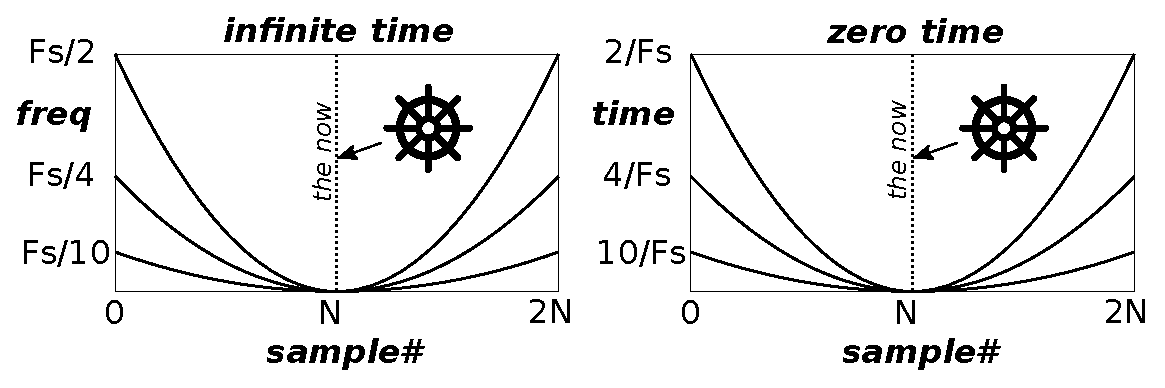
\includegraphics[width=0.95\linewidth]{../source/parabola_e}
    \caption[Hypothetical Parabolic Frequency Chirp]{Parabolic Chirp}
\end{figure}

\begin{equation} \label{eq:parabolic}
f(t, t_{now}) = k \cdot (t - t_{now})^2
\end{equation}

The singularity could have zero time instead of zero frequency:

\begin{equation} \label{eq:parabolictime}
f(t, t_{now}) = k / (t - t_{now})^2
\end{equation}

A problem with this model is that the cosine is periodic.
If signals were present, one would expect periodic artifacts that would have
been detected by now. Frequency analysis of electronic noise
from $10^{-6}$ Hz to over 1 THz can be found in the literature.
However, it's only a problem if the chirp is repeating in the same timeline.
The chirps could be on uncorrelated timelines in the multiverse.

A chirp would only be detectable if its timeline enters the realm of phenomena
that actually occur.
Considering outcomes as arising from probabilistic fields,
the most likely probabilities should produce the strongest signals.
Each chirp could be imagined as a conic section intersecting the light cone of
a Minkowski Space Time diagram. 
Whether the conic section is parabolic, hyperbolic or elliptical, within the 
system passband (which is assumed to be very limited) it looks parabolic.

Tests found that the signal was difficult to detect when it was more than 
10 dB below the noise.
Although it's an interesting possibility,
the low sensitivity of the conic section model doesn't engender much confidence
in its ability to model nature.

However, if the observer interacts through consciousness with what is being
observed, interfering signals could be worked around.
The system would compensate for them as a sort of forward error correction.
If the living system can detect the signal, perhaps the algorithm can too.
The sensor would have to interact with the living system to see what it sees.
Otherwise, the uncorrelated noise would swamp it.

\subsection{Information in the Noise}

Since chirps are bounded in time, a single chirp has a finite
existence within a practical bandwidth. 
It corresponds to a discrete impulse in the relative time domain,
or one symbol of information.
The idea of consciousness as time quanta may be useful here.
The act of being is a stream of consciousness that could have corresponding
streams of pulse-coded information, a kind of informational counterpart to DNA.
The impulse stream would be decoded for its information content.

To establish a notation and unit of measurement for quantum frequency,
let the ``warp factor'' $\omega$ be in units of $e$, the
mathematical constant derived by Leonhard Euler in the 1720s, per unit time.
The pronunciation may be ``e's per second'' for e/s, for example.

Note that 1.0 e/s is very close to twice the Golden Ratio $(\Phi=1.618:1)$,
so one should be careful when making assumptions about Golden Ratio relationships
in nature.

%%%%%%%%%%%%%%%%%%%%%%%%%%%%%%%%%%%%%%%%%%%%%%%%%%%%%%%%%%%%%%%%%%%%%%%%%%%%%%%%
\subsection{A Spiral Conceptual Model}

\begin{figure}[h]
    \centering
    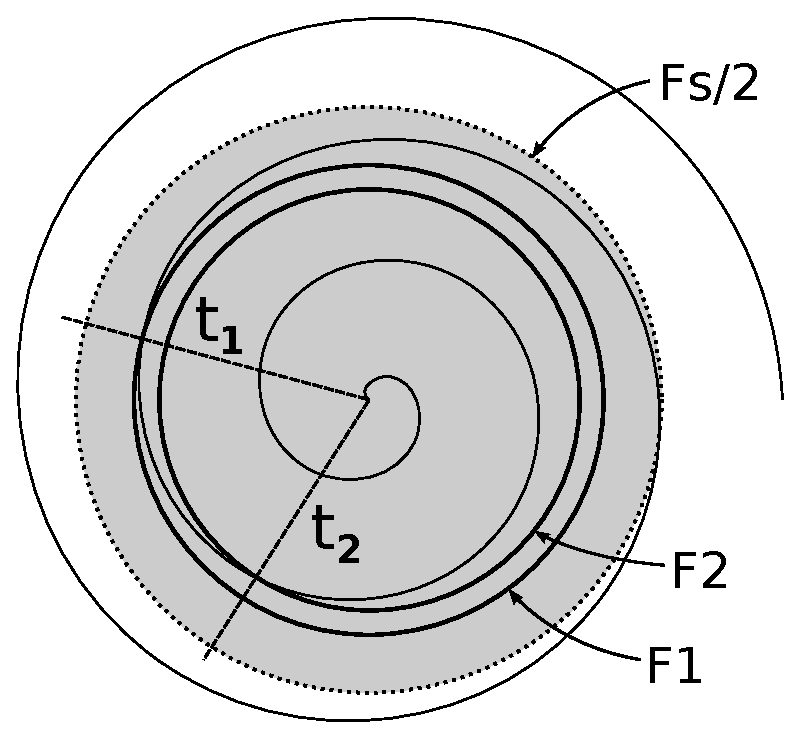
\includegraphics[width=0.7\linewidth]{../source/spiral_e}
    \caption[Quantum to Relative Time Relation]{Log polar plot of exponential chirp}
    \label{fig:spiral}
\end{figure}

Resonant signals in the quantum time domain could be re-mapped to relative time
and demodulated by correlating a series of fast Exponential Chirp Transforms (ECT). 
The spiral model needs $\omega$ to be real for Eq. \ref{eq:wp} to be self-similar.

The correlation effect can be visualized as a spinning logarithmic spiral
illuminated by a strobe light. When the strobe frequency matches the rate
constant of the spiral(s), it appears to be standing still.
Otherwise, it's a blur.

The relationship between quantum time and relative time can be thought of as a
2D plot in log-polar format.
Log-polar format renders a logarithmic spiral as a linear (Archimedean) spiral.
The spiral's radius is $\rho = k\theta$, where $k$ is a rate constant.
$\rho$ can represent either time or frequency by flipping the sign of $k$.
For purposes of signal processing, let $\rho$ represent log frequency and
$\theta$ relative time.

Log-polar mapping has proven useful in machine vision \cite{Bonmassar}
because it approximates the primate visual map \cite{Schwartz}.
Humans are visual thinkers, so their waking consciousness should map onto the
log-polar structure of quantum time signaling.

Fig.~\ref{fig:spiral} plots an exponential chirp in log-polar format.
A line can be drawn outward from the center of the spiral, crossing it at
multiple points.
The line rotates clockwise (in the case of downward chirp) at a step size
(from $t_1$ to $t_2$) corresponding to the oversampling rate.
For example, if the oversampling rate is 36 (each input value is used 36 times),
the step size is $10^{\circ}$.
Each angular sweep of the unit circle
(beginning and ending at line $t_1$ or $t_2$)
represents the input to a version of the Mellin transform called the
``Exponential Chirp Transform'' (ECT) \cite{Bonmassar}, which is
basically a Fourier Transform with time-warped input.

The transform's frequency domain output is along line $t_1$ or $t_2$ from
approximately $\rho$ = 0 to Fs/2, where Fs/2 (the Nyquist frequency)
is shown by the dashed circle.
The radius of the circle represents the approximate bandwidth of the system.
Not all of the circle is used: Anti-aliasing cuts off before Fs/2, while signal
near the center is too spread out to be useful.

The ECT time-warps the chirp signal, which represents a single ``quantum tone''.
In the $360^{\circ}$ sweep at line $t_1$,
the chirp is time-warped to a tone F1 in relative time.
A time $t_2-t_1$ later, at line $t_2$,
it's time-warped to a tone of frequency F2.
Time warping is exponential.
Note that ``exponential time warping'' is different from ``dynamic time
warping'', a popular means of pattern-matching mostly linear signals.

A convenient side effect of time warping is to transform interference
(periodic signals) into wide-band noise.
The usual frequency peaks of EEG and HRV are thus reduced.
Periodic signals could be notched out as needed by appropriate filters
to further reduce their interfering effect.

Being logarithmic, quantum time has the property of frequency going as
$-\tau$ rather than $1/t$.
To change between time and frequency, just flip the sign of the exponent.
Tones are mirror images of time.
Signal processing is more convenient in terms of frequency,
so that is the focus of this paper.

%%%%%%%%%%%%%%%%%%%%%%%%%%%%%%%%%%%%%%%%%%%%%%%%%%%%%%%%%%%%%%%%%%%%%%%%%%%%%%%%
\subsubsection{\label{sec:level1}The Spiral Transform}

The basic data flow of signal conversion from one time domain to another
$(\tau \leftrightarrow t)$ is shown in Fig.~\ref{fig:sled}.
The conversion algorithm slides along the input and output data streams,
forward in time.
Data is processed in overlapping chunks.
In other words, after a block of processing,
the sliding part of Fig.~\ref{fig:sled} shifts slightly to the right.
In proportion to the amount of shift,
new input stream is exposed and new output stream is sent out.
The I/O streams are low-bandwidth compared to the compute-intensive
processing block.

\begin{figure}
    \centering
    \includegraphics[width=0.95\linewidth]{../source/sled_e}
    \caption[Quantum to Relative Time Translation Flow]{Inter-domain data flow}
    \label{fig:sled}
\end{figure}

There are two use cases: demodulation and modulation.
For demodulation $(\tau \rightarrow t)$, the input stream is in the quantum
time domain and the output stream is in the relative time domain.
The input stream consists of real numbers. It gets exponentially time-warped
to convert chirps to tones and fed through a FFT (Fast Fourier Transform).
The FFT result is linearized with respect to the quantum domain by exponentially
warping it and accumulating it in a correlator to
include many instances of the same incoming chirp.

For modulation $(t \rightarrow \tau)$, the input stream is in the relative time
domain and the output stream is in the quantum time domain.
It's the demodulation process in reverse.
The usual use case is demodulation, so that will be the focus of the paper.

%%%%%%%%%%%%%%%%%%%%%%%%%%%%%%%%%%%%%%%%%%%%%%%%%%%%%%%%%%%%%%%%%%%%%%%%%%%%%%%%
\subsubsection{\label{sec:level1}The Parabolic Transform}

A spectrum analyzer for the parabolic model is simpler than one for the spiral model.
The frequency chirps shown in Fig. \ref{fig:parabolic} is time-warped by 
re-sampling so as to shift the frequencies up to their respective
$F_S/2$, $F_S/4$, and $F_S/10$. This is fed through a Fourier Transform to produce
a new column of pixels for each new slice of raw input data.


\section{Spiral Model Demodulation}

\begin{figure}
    \centering
    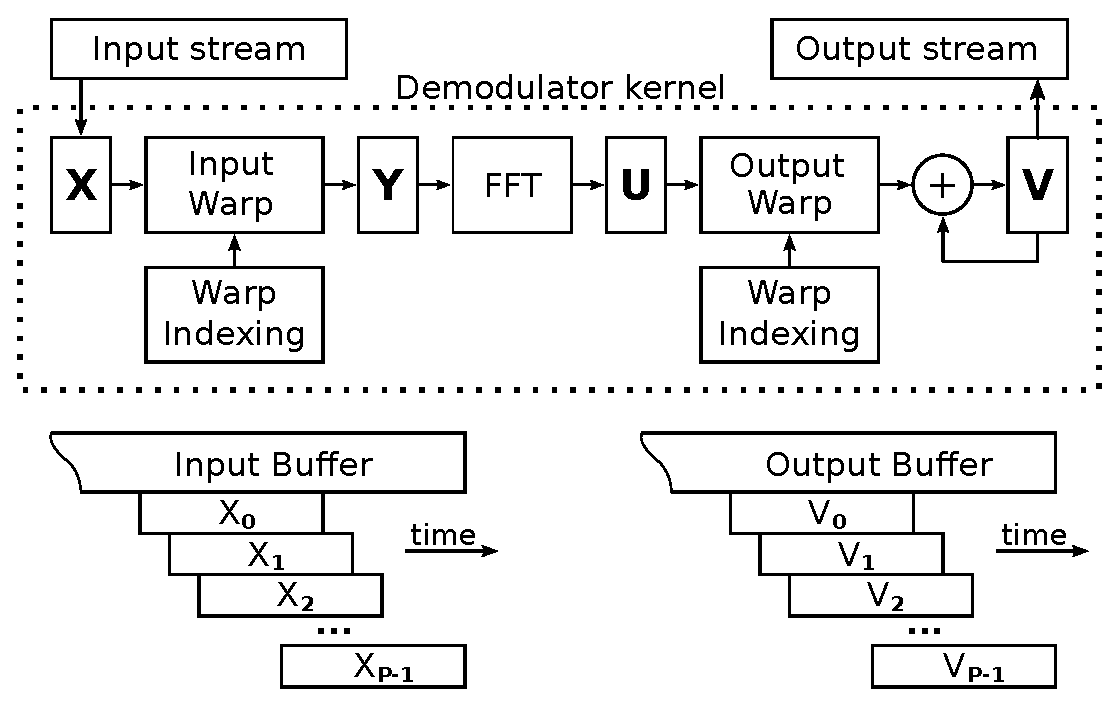
\includegraphics[width=0.95\linewidth]{../source/demod_e}
    \caption[Quantum to Relative Time Demodulation]{Demodulation data flow}
    \label{fig:demod}
\end{figure}

The mathematics of signal conversion, besides FFT, is mainly College Algebra.
The algorithm can be coded by a typical programmer or engineer with the help
from some math tricks and perhaps working around the bugs in my thinking.

%%%%%%%%%%%%%%%%%%%%%%%%%%%%%%%%%%%%%%%%%%%%%%%%%%%%%%%%%%%%%%%%%%%%%%%%%%%%%%%%
\subsection{Reference Chirp}

The most important part of a software ecosystem is its test code.
The test code for QTDSP generates a reference chirp.
That chirp is the basis for the demodulation algorithm.

Let R be a scaled version of $\omega$.
Let N be the size of the Fourier Transform, which is an exact power of two.
Typically, it's between 256 and 16384. 
Stepping $n$ from 0 to N-1,

\begin{equation}  \label{eq:tc}
f(n) = f_0 \cdot exp\left(\frac{nR}{N}\right)
\end{equation}

Computing many sequential points of transcendental functions tends to be slow.
It's better to come with a fast algorithm. With some luck, it will also illuminate   
the problem of fast signal demodulation.

Stepwise exponential growth or decay can be handled by a multiply operation.
Let $b$ be the step size for the multiplier.
Setting $e^R = (1 + b)^N$,
\begin{equation}
b = e^{R/N} - 1
\end{equation}

For each iteration:
\begin{equation}
f_{n+1} = f_n \cdot (1 + b)
\end{equation}

Since $R/N \ll 1$, the first term or two of the Maclaurin series expansion of the
exponent function is enough for a good approximation.
So, $b$ is very close to $R/N$.

%%%%%%%%%%%%%%%%%%%%%%%%%%%%%%%%%%%%%%%%%%%%%%%%%%%%%%%%%%%%%%%%%%%%%%%%%%%%%%%%
\subsection{Input Warping}

The downsampling process of Fig.~\ref{fig:demod} translates the sample pitch of
$\vec{X}$ to the sample pitch of $\vec{Y}$ using an exponential sweep.
In the industry, this is known as exponential time-warping.
The input time warp re-samples input data such that a reference chirp would get
translated to a constant-period sinusoid.

An exponential chirp sweeps from $f_0$ to $f_1$ in a time $t$.
M points of $\vec{X}$ get mapped onto N points of $\vec{Y}$, where $M < N$.
Re-sampling is done on N points (of $\vec{Y}$) at a time where the respective indices of
$\vec{X}$ and $\vec{Y}$ are $\delta$ and $i$.
$\vec{X}$ is swept from $\mathbf{X}_0$ to $\mathbf{X}_M$
or $\mathbf{X}_M$ to $\mathbf{X}_0$.

Let $\lambda$ be the sample pitch of $\vec{X}$.
It will increase or decrease exponentially and should have a maximum value of 1.

This causes a chirp of matching R to be re-sampled to the upper frequency
(either $f_0$ or $f_1$ depending on the sign of R).
Given output index i, input sample index $\delta(i)$ is the accumulated sum of
$pitch(i)$ where $pitch$ decreases exponentially from 1.0
or increases exponentially toward 1.0.
In the latter case, the initial $pitch$ can either be determined from a dummy
run of the resampling algorithm or analytically.
It's $e^{M \cdot R/N}$. 
M is derived from a geometric progression in Eq. \ref{eq:M_N0}.

\begin{equation}  \label{eq:M_N0}
N = \sum_{k=1}^{M} e^{|R| \cdot (k-1)/N} = \frac{1 - e^{|R| \cdot M/N}}{1 - e^{|R|/N}}
\end{equation}

\begin{equation}  \label{eq:M_N}
M = \frac{N}{|R|} \cdot\ ln\left( 1 - N(1-e^{|R|/N}) \right)
\end{equation}

An analytical expression of the re-sampling function ($i$ to $\delta$)
was over my head, but it's easily expressed as an algorithm.
Interpolating from a fractional $\vec{X}$ index in this example (WarpIn listing)
is done by cubic interpolation using a Catmull-Rom spline.
Given four points $y_0, y_1, y_2, y_3$, a cubic polynomial describes the curve
passing through all four points whose slope matches up between adjacent segments.
With $x$ ranging from 0 to 1 indexing the point on $[y_1, y_2]$.

\begin{equation}  \label{eq:cubic}
f = a_0 \cdot x^3 + a_1 \cdot x^2 + a_2 \cdot x + a_3
\end{equation}

\begin{lstlisting}[float,floatplacement=H]
float WarpIn(
  float* out,        // output stream
  float* in,         // input stream
  int length,        // points in output stream
  double delta,      // starting input index, 0 to 1
  double pitch,      // exponential input sample pitch
  double b,          // exp rate of change of pitch
  double amplitude,  // starting amplitude
  double fcomp)      // decay rate of amplitude
{
  float y0 = *in++;
  float y1 = *in++;
  float y2 = *in++;
  float y3 = *in++;
  // coefficients for first y1-y2 segment of the curve
  float a0 = -0.5 * y0 + 1.5 * y1 - 1.5 * y2 + 0.5 * y3;
  float a1 = y0 - 2.5 * y1 + 2.0 * y2 - 0.5 * y3;
  float a2 = -0.5 * y0 + 0.5 * y2;
  float a3 = y1;
  for (int i = 0; i < length; i++) {
    float x = delta; // between 0 and 1 on y1-y2 path
    float sum = x * (x * (x * a0 + a1) + a2) + a3;
    *out++ = sum * amplitude; // deemphasize low end
    delta += pitch;
    if (delta >= 1.0) {
      delta -= 1.0;
      pitch += pitch * b;
      amplitude += amplitude * fcomp;
      y0 = y1;       // stepped into the next segment
      y1 = y2;
      y2 = y3;
      y3 = *in++;
      a0 = -0.5 * y0 + 1.5 * y1 - 1.5 * y2 + 0.5 * y3;
      a1 = y0 - 2.5 * y1 + 2.0 * y2 - 0.5 * y3;
      a2 = -0.5 * y0 + 0.5 * y2;
      a3 = y1;
    }
  }
  return pitch;
}
\end{lstlisting}

Regardless of the sign of $R$, the input warp shifts the corresponding chirp
to the lesser of $f_0$ and $f_1$. Let $\gamma$ be the highest frequency component in the
time-warped input:

\begin{equation} \label{eq:gamma}
\gamma = \frac{N}{2} \cdot \frac{1}{1 + |R|}
\end{equation}

Note: The effect of S on $\gamma$ hasn't been tested yet.

Input interpolation produces noise artifacts, as you would expect.
They get spread broadly across the spectrum above the region of interest.
Figure \ref{fig:inwarpspec} shows the output power spectrum (10 dB/div) of
the warp function. The test chirp decays in frequency exponentially from
$0.45 F_S$ with $R=-2$.
A 4096-point Fast Fourier Transform omits the window function so you can
see the distribution of noise artifacts to the right of the peak.

\begin{figure}
  \includegraphics[width=\linewidth]{../source/inwarpspec.png}
  \caption{$f_1$ peak of warped exponential chirp, with artifacts.}
  \label{fig:inwarpspec}
\end{figure}

That's a great relief because it removes any need for much more
compute-intensive resampling algorithms. Warping may be kept simple and fast.


%%%%%%%%%%%%%%%%%%%%%%%%%%%%%%%%%%%%%%%%%%%%%%%%%%%%%%%%%%%%%%%%%%%%%%%%%%%%%%%
\subsection{FFT}

After $\vec{X}$ is time-warped into $\vec{Y}$, $\vec{Y}$ is processed by a
Fast Fourier Transform and converted to data set $\vec{U}$ containing N/2
frequency bins. Not all of them are used.
Outputs above $\gamma$ (Eq. \ref{eq:gamma}) are ignored.

$\vec{Y}$ and $\vec{U}$ may share the
same physical memory if the FFT is performed in place.
The output of the FFT is converted to the square of the magnitude for use in
RMS averaging, so square root is not needed.

A window function $w(n)$ is applied to Y before performing the FFT.
Hann and Nuttall windows are both good functions, with a tradeoff between
peak spreading and dynamic range.
Eq. \ref{eq:hann} is the Hann window function.

\begin{equation} \label{eq:hann}
w(n) = \frac{1}{2}\left(1 - cos\left( \frac{2\pi n}{N-1} \right)\right)
\end{equation}

Given N input points, output indices up to $\frac {0.5 \cdot N}{1 + |R|}$
are used for further processing.


%%%%%%%%%%%%%%%%%%%%%%%%%%%%%%%%%%%%%%%%%%%%%%%%%%%%%%%%%%%%%%%%%%%%%%%%%%%%%%%%
\subsection{Output Warping}

$\vec{U}$ is upsampled to form time-domain signal $\vec{V}$.
Let $\epsilon$ and $j$ be the respective indices of $\vec{U}$ and $\vec{V}$.
The maximum usable value of $\epsilon$ is $\gamma$ (Eq. \ref{eq:gamma}).
Integer index $j$ steps one at a time while $\epsilon$ decays exponentially.

Warp indexing uses the relation:
\begin{equation}
\epsilon = \gamma e^{\omega(t - \tau)}
\end{equation}

Time $t$ (scaled to match the output stream's sample rate) sweeps from $\tau$
in the opposite direction of R's sign,
causing the exponent to start at 1 and decay downward.

$j$ sweeps downward from $\gamma(N/2-1)$.
Index $\epsilon(j)$ is independent of R.

\begin{equation}  \label{eq:eps_j}
\epsilon(j) = \gamma e^{-kj/N}
\end{equation}

The desired difference between $\epsilon(0)$ and $\epsilon(1)$ in
Eq. \ref{eq:eps_j} is $1$. $\epsilon(0) = \gamma$
and $\epsilon(1) = \gamma e^{-k/N}$,
which gives a $k$ of about $-2|R|$:

\begin{equation}  \label{eq:k}
k = N \cdot ln \left(1 - 2 \cdot \frac{|R| + 1}{N} \right)
\end{equation}

The exponential decay of $\epsilon$ can be handled by repeated multiplication,
one per $\vec{U}_\epsilon$ fetch.
The exponential sweep needs a small correction factor to have a base of exactly
$e$.
%\frac{N}{2} \cdot (1 - e^{-k})
Setting $e^{k} = (1 + \zeta)^{N}$,
\begin{equation}
\zeta = e^{k/N} - 1
\end{equation}

Sample C code for the output warp:

\begin{lstlisting}[float,floatplacement=H]
static void WarpOut(
  float* out,               // output stream (V)
  float* in,                // input stream (mag^2)
  int length,
  double gamma,             // max epsilon index
  double zeta,              // rate of change of gamma
  float fcomp)              // decay rate of amplitude
{
  int idx0 = (int)gamma;
  in = &in[idx0 + 1];       // -> first point
  double epsilon = gamma;
  float amplitude = 1.0f;
  float y1 = *in--;
  float y0 = *in--;
  float a0 = y1 - y0;
  float a1 = y0;
  for (int i = 0; i < length; i++) {
    float idx1 = idx0;
    float x = gamma - idx0; // between 0 and 1 on y0-y1
    float sum = x * a0 + a1;
    *out++ = sum * amplitude; // deemphasize low end
    amplitude += amplitude * fcomp;
    gamma += gamma * zeta;  // epsilon exponentially decays
    idx0 = (int)gamma;
    if (idx0 != idx1) {
      y1 = y0;              // stepped into the next segment
      y0 = *in--;
      a0 = y1 - y0;
      a1 = y0;
    }
  }
}
\end{lstlisting}


%%%%%%%%%%%%%%%%%%%%%%%%%%%%%%%%%%%%%%%%%%%%%%%%%%%%%%%%%%%%%%%%%%%%%%%%%%%%%%%%
\subsection{Correlation}

Let $H_X$ be the integer number of new X samples per conversion.

Let $H_V$ be the real number of output samples per conversion.
Combining Eq. \ref{eq:gamma} and Eq. \ref{eq:k} gives:

\begin{equation}  \label{eq:hv}
H_V = H_X \cdot \frac{R}{N} \cdot \frac{R}{|R| + 1}
          \cdot \frac{-1}{ln(1 - \frac{2|R|}{N})}
\end{equation}

Since $\epsilon$ is always positive, the upchirp case of $R>0$ needs to have its
j index mirrored by using $\vec{U}_{v-j}$, where v is the maximum j such as (15/32)N.
The warp output is added to $\vec{V}$ memory as described below, indexed from the
top or bottom of the active region of V.

Warped $\vec{U}$ is added to output buffer $\vec{V}$ by summation,
staggered in time (by $H_V$ samples) for each processing block.
When the downsampler's R value matches the chirp rate of an incoming chirp,
multiple peaks in the warped FFT output correlate in the output stream to
produce a corresponding output pulse in the $\vec{V}$ stream.
A more complex signal such as overlapping and/or modulated chirps will produce
pulse trains and/or modulation envelopes in the $\vec{V}$ stream.

$\vec{U}$ is in logarithmic format so that summing a bunch of them is basically 
repeated multiplication.
It's cheaper than actual multiplication and less subject to overflow.
Multiplying (or summing logs) of linearized spectra is a form of cross-correlation.
The sum can be normalized with a scale that's the inverse of the V oversampling:

\begin{equation}
scale = -H_X \cdot \frac{R^2}{ln(1 - \frac{2|R|}{N})}
\end{equation} % (n / 2) / (1 + fabs(r))

\begin{figure}
    \centering
    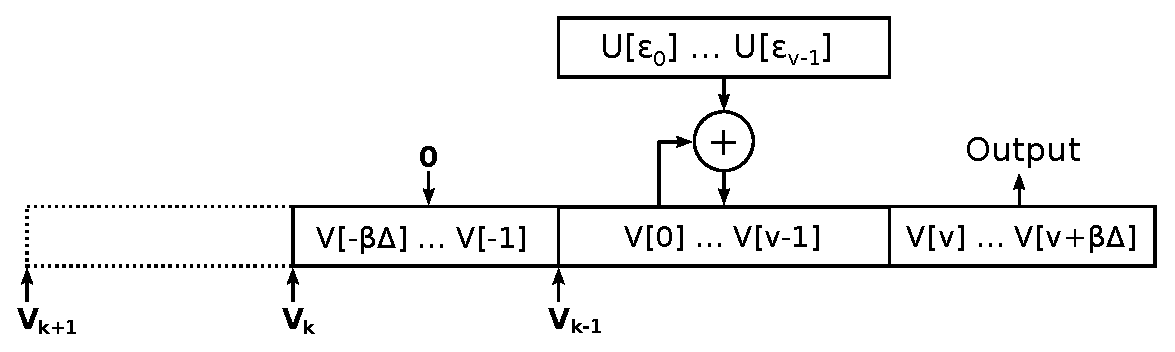
\includegraphics[width=0.99\linewidth]{../source/wbuf_e}
    \caption[$\vec{V}$ correlation]{Correlation of $\vec{V}$}
    \label{fig:wbuf}
\end{figure}

Fig.~\ref{fig:wbuf} shows the output correlator, another view of buffer $\vec{V}$.
The output stream flows from left to right,
being initialized to 0 outside the accumulation region.
After $U_\epsilon$ is added to $\vec{V}$, the $V_0$ index moves $H_V$ points
to the left, leaving $H_V$ newly minted output points.

Elements of $\vec{V}$ are accumulated squares of magnitudes.
An attempt was made to accumulate vectors,
with the idea that the phase rotations might sync up,
but it didn't work in simulation.
So, angle data from the FFT is discarded.

\section{Parabolic Model Demodulation}

The parabolic time model is simpler than the spiral model.
There's no correlator. A spectrum analyzer is also easier to build.

%%%%%%%%%%%%%%%%%%%%%%%%%%%%%%%%%%%%%%%%%%%%%%%%%%%%%%%%%%%%%%%%%%%%%%%%%%%%%%%%
\subsection{Reference Chirp}

The parabolic chirp has a frequency that starts at $F_0$ and ends at 0.
Its frequency forms half of a parabola when $N$ points are plotted.

%%%%%%%%%%%%%%%%%%%%%%%%%%%%%%%%%%%%%%%%%%%%%%%%%%%%%%%%%%%%%%%%%%%%%%%%%%%%%%%%
\subsection{Input Warping}

The downsampling process of Fig.~\ref{fig:demod} translates the sample pitch of
$\vec{X}$ to the sample pitch of $\vec{Y}$ using a parabolic sweep.
The input time warp re-samples input data such that a reference chirp would get
translated to a constant-period sinusoid.

M points of $\vec{X}$ get mapped onto N points of $\vec{Y}$, where $M = 0.468N$.
The chirp's $F_0$ gets down-sampled by a factor of 3.53 to match $F_1$,
the frequency at $X[M]$.
As with the spiral model, such down-sampling is well-behaved.
Upsampling $F_1$ to $F_0$ would be more difficult and need anti-aliasing filtering.

Rather than showing a mathematical derivation,
a code listing of the time warping tells all. 
Cubic interpolation via Catmull-Rom spline is again used.

\begin{lstlisting}[float,floatplacement=H]
void ParabolicWarp(
  float* out,       // output stream
  float* in,        // input stream
  int n,            // points in output stream
  float pitch)      // exponential input sample pitch
{
  float y0, a0, a1, a2, a3;
  float y1 = *in++;
  float y2 = *in++;
  float y3 = *in++;
  float x = 0;      // between 0 and 1 on y1-y2 path
  float dp = n;     // dharma point is at right edge
  float dp0 = sqrtf(pitch) * dp;
  pitch = 1.0;
  for (int i = 0; i < n; i++) {
    x += pitch;
    if (x >= 1.0) { // stepped into the next segment
      x -= 1.0;
      float s = dp0 / dp;
      pitch = s * s;
      dp--;
      y0 = y1;
      y1 = y2;
      y2 = y3;
      y3 = *in++;
      // coefficients for y1-y2 segment of the cubic curve
      a0 = -0.5f * y0 + 1.5f * y1 - 1.5f * y2 + 0.5f * y3;
      a1 = y0 - 2.5f * y1 + 2.0f * y2 - 0.5f * y3;
      a2 = -0.5f * y0 + 0.5f * y2;
      a3 = y1;
    }
    *out++ = x * (x * (x * a0 + a1) + a2) + a3;
  }
}
\end{lstlisting}

After $\vec{X}$ is time-warped into $\vec{Y}$, $\vec{Y}$ is processed by a
Fast Fourier Transform and converted to magnitude data $\vec{U}$ containing N/2
frequency bins. Not all of them are used.
Outputs above $F_S / 7$ are ignored.

Given N input points, output indices up to $F_S / 7$
are used for further processing.

%%%%%%%%%%%%%%%%%%%%%%%%%%%%%%%%%%%%%%%%%%%%%%%%%%%%%%%%%%%%%%%%%%%%%%%%%%%%%%%%
\subsection{Spectral Display for Parabolic Time}

The FFT output can be used to form a column of heat-mapped pixels on a display.
Each subsequent conversion forms another column.
$H_X$ samples are appended to $\vec{X}$ for each new conversion.
A GPU would typically run hundreds of warps and FFTs in parallel to produce a
2D image as a single processing block.

Since there is no correlation step, the parabolic chirp is smeared across the
output image.
Figure \ref{fig:p4kbw3} illustrates the image produced by a test waveform.
$F_0$ is $F_S/2$.
At $F_0$, the smear is thinnest.
The high frequency components of the smear are the most pronounced at $F_0$.
A 2D FFT can be used to help pick out the location of the chirp.

\begin{figure}
  \includegraphics[width=0.8\linewidth]{../source/p4kbw3.jpg}
  \caption{Parabolic chirp 3dB below noise.}
  \label{fig:p4kbw3}
\end{figure}


%\input{../source/qtdsp_mod}
\section{Testing}

The demodulation algorithm was tested by coding the algorithm in C (as a console
application) and instrumenting it to display variables,
save arrays to files, and benchmark the various stages.
KissFFT is used as the FFT.
A GPU would be much faster and will be used in further studies.

\subsection{Demodulation to Image}

The demodulation algorithm looks at the signal bandwidth between about
$\gamma F_S/5$ and $\gamma F_S/2$ where $\gamma$ is between 0.25 and 1.

Figure \ref{fig:chirpTest1} shows a spectrogram image of a noisy test signal
with R on the vertical axis.
$R=-0.2$ is at the top and $R=-0.78$ is at the bottom.
The output rates for each R are normalized (stretched at the low end)
to fit the image.
This gives the top of the image a fuzzy appearance.
A test signal was used to demonstrate detection of a chirp at
$R=-0.5$ and $N=4096$.
The chirp amplitude is 1/10 of the noise amplitude.
\begin{figure}
  \includegraphics[width=\linewidth]{../source/chirp42m.jpg}
  \caption{Chirp power 20dB below noise.}
  \label{fig:chirpTest1}
\end{figure}

Noise has a cobweb-like look. A chirp shows up as a peak among the cobwebs.
To pick the chirp out of this mess, the peak is stored for each R value.
Figure \ref{fig:chirpRvalues1} shows the peak R values for a test chirp with a
power level 20, 25 and 30 dB below random noise.
\begin{figure}
  \includegraphics[width=\linewidth]{../source/Rpeaks.png}
  \caption{Peak power versus R}
  \label{fig:chirpRvalues1}
\end{figure}

\subsection{Test on Stock Trades}

An intriguing possibility is that
group consciousness produces visible artifacts in stock market data.
If such signals exist (yeah right), great. Let's get rich.
If not, this test will save you some work because you know you've got to try it.

Seconds-resolution sample data, SPY_SECOND_TRADE.csv downloaded from QuantQuote, 
shows the price history of a stock over a trading day from 4:00 AM to 7:59 PM.
A simple C utility (stock.c) converts the CSV file to a usable format.
The interval between data points is much longer than a second at the beginning
and end of the day and about a second during active trading. 
To handle intervals longer than one second,
data is linearly interpolated to produce one point per second.
Anomalous spikes are filtered out to reduce the noise level.
16 hours is 57600 seconds, enough for a 14K-wide bitmap.
Data at the beginning of the day is rather sparse, but it's not really visible.


\section{Summary}

Signals that appear to be pure noise may contain hidden signals regarding non-local consciousness.
These signals could be analyzed to ``instrument the soul''.
Follow-up work to be done includes:

\begin{itemize}
	\item Add features to the QTSA app to facilitate signal identification.
	\item Analyze existing experimental data to search for new signals.
	\item Develop new sensor technologies using quantum and spin effects.
\end{itemize}

The social impetus for such work is to repair the dysfunction introduced by
new technologies such as social media and pseudo-anonymous communications.
Instrumenting the soul would provide a new way of interacting that is completely open and honest.

QTDSP could be key to solving the wetiko disease epidemic that has plagued humanity for the
last several millenia. 

\subsection{Peace on Earth}

The motivation behind QTDSP is to solve the world's most vexing social problems by
using technology to decapitate the Medusa.
At the root of problems such as social injustice, political malfeasance,
the threat of fascism, financial corruption, totalitarianism,
endless war, the threat of nuclear war, and our inability to address climate change
is a form of psychic blindness called \emph{wetiko}.

\emph{Wetiko} is an Algonquin word (\emph{windigo} in Ojibwa, \emph{wintiko} in Powhatan)
for a cannibalistic spirit that is driven by greed, excess, and selfish consumption.
It is the ``disease caused by yellow metal''.

This contagious psycho-spiritual disease of the soul, a parasite of the mind, is currently
being acted out en masse on the world stage via a collective psychosis of titanic
proportions \cite{Levy}.

Wetiko works through the blind spots of the unconscious and the projective tendencies of
the mind so as to hypnotize us via our mind’s own creative power to shape reality.
It renders people oblivious to their own madness and compels them to act
against their own best interests.
This mind-virus only has power over us to the extent it is not seen, so the way to heal
it is to see how it operates, both out in the world and within our own mind.

Electronic devices that detect and display wetiko can lead to its annihilation.
The productive capacity of the leading device manufacturers could literally change
the world, in a holistic and divine way, almost overnight.

Besides the development of sensors, which looks promising given the state of quantum
computer technology, a mathematical model of time is needed to translate signals
into something digestible by AI and pattern matching algorithms.




\bibliography{../source/qtdsp}% Produces the bibliography via BibTeX.

\end{document}
%
% ****** End of file qtdsp.tex ******
